%%%% CAPÍTULO 2 - REVISÃO DA LITERATURA (OU REVISÃO BIBLIOGRÁFICA, ESTADO DA ARTE, ESTADO DO CONHECIMENTO)
%%
%% O autor deve registrar seu conhecimento sobre a literatura básica do assunto, discutindo e comentando a informação já publicada.
%% A revisão deve ser apresentada, preferencialmente, em ordem cronológica e por blocos de assunto, procurando mostrar a evolução do tema.
%% Título e rótulo de capítulo (rótulos não devem conter caracteres especiais, acentuados ou cedilha)
\chapter{Referencial te\'orico}\label{cap:referencialTeorico}

Uma forma de tratar o referencial teórico é definir como título de capítulo o assunto macro e relevante relacionado ao trabalho e o texto é dividido em subtítulos (seções e subseções), conforme necessário. Essa forma é preferida por deixar explícito o assunto a ser tratado e que o mesmo é a fundamentação do trabalho \footnote{Teste de nota de rodapé 3.}. 

Outra forma de tratar esse capítulo é denominá-lo referencial teórico e dividi-lo em seções e subseções ou com um único texto os assuntos que fornecem o suporte teórico para o trabalho. Essa forma pode ser utilizada quando assuntos distintos fundamentam o trabalho e é difícil incluí-los sob uma mesma denominação de capítulo \footnote{Teste de nota de rodapé 4.}.

O embasamento teórico se refere ao(s) assunto(s) principal(is) relacionado(s) ao objeto de pesquisa para o qual o trabalho traz alguma contribuição ou que é utilizado como referência conceitual para o desenvolvimento do proposto no trabalho. O assunto pode fornecer a fundamentação (suporte teórico) para a ideia do sistema, para definir claramente o problema, para explicitar a solução, para a forma de resolução; referir-se aos conceitos e teorias relacionados ao sistema desenvolvido, sobre tecnologias e metodologias específicas utilizadas na definição do sistema e na sua implementação.

Exemplos:

Conceitos da orientação a objetos fazem parte do referencial teórico se o uso intensivo da orientação a objetos é o principal embasamento do trabalho; ou se a principal contribuição do trabalho está relacionada à orientação a objetos, seja em termos de agregar conhecimento nessa área ou à forma de usar os seus conceitos.

Sistemas distribuídos pode ser o assunto do embasamento teórico se o resultado do trabalho for um sistema distribuído. O mesmo pode ocorrer com sistemas cliente servidor, sistemas de informações gerenciais, de apoio à decisão, para web e etc.

Se o desenvolvimento de um sistema para biometria for o objeto do trabalho, o referencial teórico se refere aos conceitos principais de biometria, aplicabilidade, exemplos de sistemas existentes, o que esses sistemas tratam, como eles são, etc.

Se um sistema web para portadores de necessidades especiais for o resultado do trabalho, o referencial teórico refere-se as quais e como são essas necessidades, outros sistemas existentes na área, como os sistemas lidam com essas necessidades e os principais conceitos por eles considerados.

O embasamento teórico pode conter os trabalhos relacionados, desde que seja relevante para o desenvolvimento do trabalho. Esse item deve ser elaborado especialmente quando se trata do desenvolvimento de algo muito específico, havendo a necessidade de um estudo comparativo. Nesse caso pode-se inserir claramente o trabalho de pesquisa no contexto dos demais autores, no sentido da contribuição da proposta na área de pesquisa em que o mesmo se insere e em relação ao que já tem pesquisado na área. 

\caixa{Atenção}{Converse com o seu orientador para ver quais seções/conteúdos devem ter neste capítulo...}

\section{Observações sobre a citações}\label{sec:formatacaoTexto}

O texto em si é dividido em títulos e subtítulos, se necessário. 

O espaçamento entre linhas é de 1,5. Os títulos das seções primárias e das demais subseções devem ser separados do texto que os precede ou que os sucede por uma linha em branco. As seções primárias devem iniciar em páginas distintas.

Com relação à paginação, todas as folhas do trabalho, a partir da folha de rosto, devem ser contadas sequencialmente, mas não numeradas. A numeração deve ser colocada a partir da primeira folha da parte textual (introdução), em algarismos arábicos, no canto superior direito da folha.

\caixa{Observação}{Se você estiver utilizando \latex, não é necessário se preocupar com formatação.}

As próximas seções comentam a respeito de citações.

\subsection{Citações}\label{subsec:citacoes}

\textbf{Citação direta:} É quando o texto utilizado é transcrito com as próprias palavras do autor. Quando curtas (até três linhas) a transcrição literal virá entre “aspas” e a referência pode ser incluída no texto junto à sentença ou frase, ou ainda ser colocada entre parênteses. Quando inclusa no texto, deve-se usar letras maiúsculas e minúsculas, com indicação da data e demais informações entre parênteses.

Exemplo de citação direta curta com autor incluso no texto: Segundo \citeonline[p. 107]{Pressman2009} o valor da informação está “diretamente ligado à maneira como ela ajuda os tomadores de decisões a atingirem as metas da organização”. Exemplo de citação direta curta com autor não incluso no texto: O autor lembra, contudo, a análise precursora de \citeonline{Pressman2009} sobre alguns aspectos limitantes das competências, ou aptidões, essenciais, que as transformam em “limitações estratégicas” \cite{Pressman2009}.

As transcrições com mais de três linhas (citações diretas longas) aparecem recuadas em 4 cm, a partir da margem esquerda, em espaço simples, tamanho 10, e a indicação da fonte é apresentada entre parênteses. 

\begin{citacao}
Na nova sociedade, chamada de capitalista: O recurso econômico básico – ‘os meios de produção’, para usar uma expressão dos economistas – não é mais o capital, nem os recursos naturais (a ‘terra’ dos economistas), nem a ‘mão-de-obra’. Ele será o conhecimento. As atividades centrais de criação de riqueza não serão nem a alocação de capital para usos produtivos, nem a ‘mão-de-obra’ – os dois pólos da teoria econômica dos séculos dezenove e vinte, quer ela seja clássica, marxista, keynesiana ou neoclássica. Hoje o valor é criado pela ‘produtividade’ e pela ‘inovação’, que são aplicações do conhecimento ao trabalho. Os principais grupos sociais da sociedade do conhecimento serão os ‘trabalhadores do conhecimento’ – executivos que sabem como alocar conhecimento para usos produtivos. \cite[p. 48]{Pressman2009}.
\end{citacao}

\textbf{Citação indireta:} É a reprodução de ideias do autor. É uma citação livre, usando as palavras de quem está escrevendo para dizer o mesmo que o autor disse no texto. Contudo, a ideia expressa continua sendo de autoria do autor consultado, por isso é necessário citar a fonte: dar crédito ao autor da ideia. Exemplo de citação indireta: O valor da informação está relacionado com o poder de ajuda aos tomadores de decisões a atingirem os objetivos da empresa\cite{Pressman2009}. Outra forma de citação indireta: \citeonline{Pressman2009} destacam ser fundamental a gestão de dados nas organizações, pois isso garantirá o funcionamento normal dos sistemas de informação, uma vez que, sem a capacidade de seu processamento, haveria problemas para a empresa executar suas atividades efetivamente.

Citações de obras que contenham até três autores, devem apresentar os sobrenomes destes separados por ponto e vírgula, como no exemplo: \cite[p. 2]{Pinto2000}. E para obras que contenham mais de três autores indica-se citar apenas o nome do primeiro autor, seguido da expressão abreviada \textit{et al.}, como no exemplo: \cite{Guimaraes2003}.

\subsection{Ilustrações, quadros e tabelas}\label{subsec:ilustracoes}

As ilustrações, quadros e tabelas devem aparecer no texto, segundo a NBR14724:2011, de forma padronizada.

Qualquer que seja o tipo de ilustração, sua identificação aparece na parte superior, precedida da palavra designativa (desenho, esquema, fluxograma, fotografia, gráfico, mapa, organograma, planta, quadro, retrato, figura, imagem, entre outros), seguida de seu número de ordem de ocorrência no texto, em algarismos arábicos, travessão e do respectivo título. Após a ilustração, na parte inferior, indicar a fonte consultada (elemento obrigatório, mesmo que seja produção do próprio autor), legenda, notas e outras informações necessárias à sua compreensão (se houver). A ilustração deve ser citada no texto e inserida o mais próximo possível do trecho a que se refere.

A fonte, ou seja, a indicação do autor da ilustração ou da publicação de onde ela foi retirada deve aparecer na parte inferior. Exemplo:

Fonte: \citeonline{Coulouris2013}. 			- quando utilizado o item original

Fonte: Adaptado de \citeonline{Coulouris2013}.	- quando o item original foi alterado

Para facilitar a inclusão de fontes, o \textit{template} em LaTeX da \gls{utfpr}, possui o comando \texttt{$\backslash$fonte\{\}}. Se este comando for deixado em branco (\texttt{$\backslash$fonte\{\}}),  ele preencherá automaticamente a fonte com o texto  ``Fonte: Autoria própria (ANO)'', sendo ANO substituído pelo ano atual. Já se o comando \texttt{$\backslash$fonte\{\}} tiver algum conteúdo (não estiver em branco), tal conteúdo será inserido na legenda da fonte e esse conteúdo pode ser uma citação. Por exemplo, o comando \texttt{$\backslash$fonte\{$\backslash$citeonline\{Coulouris2013\}\}} gerará o texto ``Fonte: \citeonline{Coulouris2013}.''. Atenção, não é necessário incluir o ponto final (``.''), no texto do comando \texttt{$\backslash$fonte\{\}}, pois isso é feito automaticamente.  

A figura também deve ser citada no texto. Primeira opção, como pode ser observado na \autoref{fig:exemplo1}. Segunda opção, como pode ser observado na Figura \ref{fig:exemplo1}.

\begin{figure}[htb]%% Ambiente figure
    %\captionsetup{width=0.55\textwidth}%% Largura da legenda
    \caption{Exemplo de figura criada a partir de um arquivo}%% Legenda
    \label{fig:exemplo1}%% Rótulo
    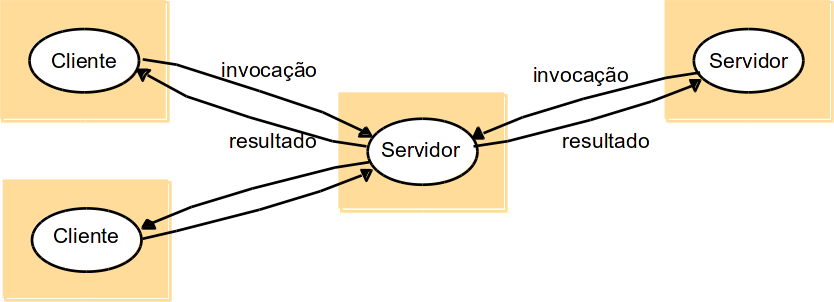
\includegraphics[scale=0.4]{cs2}%% Dimensões e localização
    \fonte{Adaptado de \citeonline{Coulouris2013}}%% Fonte
\end{figure}

Utilizando o pacote \textit{subfig} é possível adicionar figuras lado a lado, como pode ser observado na \autoref{fig:exemplo2}.

\begin{figure}[htb]
    \caption{Telas de cadastro de Paciente: (a) Cadastro Paciente, (b) Cadastro Paciente 2} 
	\label{fig:exemplo2}
	\centering
	\subfloat[Cadastro Paciente]{
		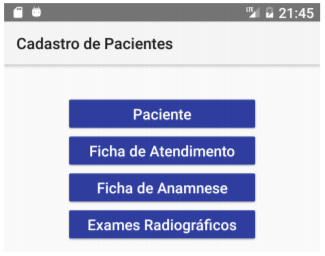
\includegraphics[scale=0.7]{cadastro-paciente}
	}\hspace{0.15cm} 
	\subfloat[Cadastro Paciente 2]{
		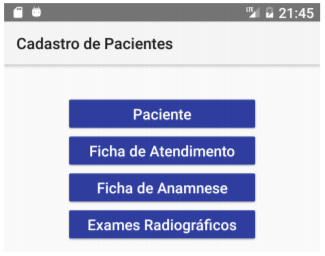
\includegraphics[scale=0.7]{cadastro-paciente}
	}
	
	\fonte{}
\end{figure}

Este modelo vem com o ambiente \texttt{quadro} e impressão de Lista de quadros 
configurados por padrão.  Este parágrafo apresenta como referenciar o quadro no texto, requisito obrigatório da ABNT. Primeira opção, utilizando \texttt{autoref}: Ver o \autoref{quad:exemplo1}. Segunda opção, utilizando  \texttt{ref}: Ver o Quadro \ref{quad:exemplo1}.

\begin{tabframed}[htb]%% Ambiente tabframed
%\captionsetup{width=0.5\textwidth}%% Largura da legenda
\caption{Materiais utilizados no desenvolvimento do sistema}%% Legenda
\label{quad:exemplo1}%% Rótulo
\renewcommand{\arraystretch}{1.5}
\begin{tabular}{|l|l|l|l|l}
\cline{1-4}
\textbf{Ferramenta/Tecnologia} & \textbf{Versão} & \textbf{Disponível em} & \textbf{Finalidade} \\ \cline{1-4}
 Teste & 1.0  & https:/teste.org & Biblioteca de Teste & \\ \cline{1-4}  
 Teste & 1.0  & https:/teste.org & Biblioteca de Teste & \\ \cline{1-4}
 Teste & 1.0  & https:/teste.org & Biblioteca de Teste & \\ \cline{1-4}
 Teste & 1.0  & https:/teste.org & Biblioteca de Teste & \\ \cline{1-4}
\end{tabular}
\fonte{}%% Fonte
\end{tabframed}


Também é possível citar tabelas no texto. Primeira opção, utilizando \texttt{autoref}: Ver o \autoref{tab:exemplo1}. Segunda opção, utilizando  \texttt{ref}: Ver a Tabela \ref{tab:exemplo1}.

\begin{table}[htb]
% Luiz - O texto do caption da tabela/quadro deve ser do tamanho da tabela, então utilize a linha a seguir para conseguir esse efeito
\captionsetup{width=0.33\textwidth}
\centering
\caption{\label{tab:exemplo1}Exemplo de tabela com uma legenda contendo um texto longo}
\begin{tabular}{cccc}
	\hline
	\textbf{Pessoa} & \textbf{Idade} & \textbf{Peso} & \textbf{Altura} \\ \hline
	Marcos & 26    & 68   & 178    \\ 
	Ivone  & 22    & 57   & 162    \\ 
	...    & ...   & ...  & ...    \\ 
	Sueli  & 40    & 65   & 153    \\ \hline
\end{tabular}
\fonte{}
\end{table}

A \autoref{tab:exemplo2} também pode ser citada no texto.

\begin{table}[htb]%% Ambiente table
\caption{Segundo exemplo de tabela com uma legenda contendo um texto muito longo que pode ocupar mais de uma linha}%% Legenda
\label{tab:exemplo2}%% Rótulo
\begin{tabularx}{\textwidth}{@{\extracolsep{\fill}}llll}%% Ambiente tabularx
\toprule
$\bsym{L}$ & $\bsym{L^2}$ & $\bsym{L^3}$ & $\bsym{L^4}$ \\
\SI{}{[m]} & \SI{}{[m^2]} & \SI{}{[m^3]} & \SI{}{[m^4]} \\ \midrule
1          & 1            & 1            & 1            \\
2          & 4            & 8            & 16           \\
3          & 9            & 27           & 81           \\
4          & 16           & 64           & 256          \\
5          & 25           & 125          & 625          \\ \bottomrule
\end{tabularx}
\fonte{}%% Fonte
\end{table}

A \autoref{tab:exemplo3} é um exemplo de tabela que ocupa mais de uma página e que foi construída pelo \gls{latex}\index{LaTeX@\latex} utilizando o pacote \texttt{longtable}.

\begin{longtable}{@{\extracolsep{\fill}}lll}%% Ambiente longtable
\caption{Possíveis tríplices para grade altamente variável\label{tab:exemplo3}} \\%% Legenda e rótulo
\toprule
\textbf{Tempo (s)} & \textbf{Tríplice escolhida} & \textbf{Outras possíveis tríplices} \\
\midrule
\endfirsthead%% Encerra cabeçalho da primeira página
\caption[]{Possíveis tríplices para grade altamente variável} \\%% Legenda
\multicolumn{3}{r}{\textbf{(continuação)}} \\
\toprule
\textbf{Tempo (s)} & \textbf{Tríplice escolhida} & \textbf{Outras possíveis tríplices} \\
\midrule
\endhead%% Encerra cabeçalho das demais páginas
\midrule
\multicolumn{3}{r}{\textbf{(continua)}} \\
\endfoot%% Encerra rodapé das demais páginas
\bottomrule
\\[-0.5\linha]
\caption*{\nomefonte: Adaptado de \citet{Smallen2014}} \\
\endlastfoot%% Encerra rodapé da última página
0      & (1, 11, 13725) & (1, 12, 10980), (1, 13, 8235), (2, 2, 0), (3, 1, 0) \\
2745   & (1, 12, 10980) & (1, 13, 8235), (2, 2, 0), (2, 3, 0), (3, 1, 0)      \\
5490   & (1, 12, 13725) & (2, 2, 2745), (2, 3, 0), (3, 1, 0)                  \\
8235   & (1, 12, 16470) & (1, 13, 13725), (2, 2, 2745), (2, 3, 0), (3, 1, 0)  \\
10980  & (1, 12, 16470) & (1, 13, 13725), (2, 2, 2745), (2, 3, 0), (3, 1, 0)  \\
13725  & (1, 12, 16470) & (1, 13, 13725), (2, 2, 2745), (2, 3, 0), (3, 1, 0)  \\
16470  & (1, 13, 16470) & (2, 2, 2745), (2, 3, 0), (3, 1, 0)                  \\
19215  & (1, 12, 16470) & (1, 13, 13725), (2, 2, 2745), (2, 3, 0), (3, 1, 0)  \\
21960  & (1, 12, 16470) & (1, 13, 13725), (2, 2, 2745), (2, 3, 0), (3, 1, 0)  \\
24705  & (1, 12, 16470) & (1, 13, 13725), (2, 2, 2745), (2, 3, 0), (3, 1, 0)  \\
27450  & (1, 12, 16470) & (1, 13, 13725), (2, 2, 2745), (2, 3, 0), (3, 1, 0)  \\
30195  & (2, 2, 2745)   & (2, 3, 0), (3, 1, 0)                                \\
32940  & (1, 13, 16470) & (2, 2, 2745), (2, 3, 0), (3, 1, 0)                  \\
35685  & (1, 13, 13725) & (2, 2, 2745), (2, 3, 0), (3, 1, 0)                  \\
38430  & (1, 13, 10980) & (2, 2, 2745), (2, 3, 0), (3, 1, 0)                  \\
41175  & (1, 12, 13725) & (1, 13, 10980), (2, 2, 2745), (2, 3, 0), (3, 1, 0)  \\
43920  & (1, 13, 10980) & (2, 2, 2745), (2, 3, 0), (3, 1, 0)                  \\
46665  & (2, 2, 2745)   & (2, 3, 0), (3, 1, 0)                                \\
49410  & (2, 2, 2745)   & (2, 3, 0), (3, 1, 0)                                \\
52155  & (1, 12, 16470) & (1, 13, 13725), (2, 2, 2745), (2, 3, 0), (3, 1, 0)  \\
54900  & (1, 13, 13725) & (2, 2, 2745), (2, 3, 0), (3, 1, 0)                  \\
57645  & (1, 13, 13725) & (2, 2, 2745), (2, 3, 0), (3, 1, 0)                  \\
60390  & (1, 12, 13725) & (2, 2, 2745), (2, 3, 0), (3, 1, 0)                  \\
63135  & (1, 13, 16470) & (2, 2, 2745), (2, 3, 0), (3, 1, 0)                  \\
65880  & (1, 13, 16470) & (2, 2, 2745), (2, 3, 0), (3, 1, 0)                  \\
68625  & (2, 2, 2745)   & (2, 3, 0), (3, 1, 0)                                \\
71370  & (1, 13, 13725) & (2, 2, 2745), (2, 3, 0), (3, 1, 0)                  \\
74115  & (1, 12, 13725) & (2, 2, 2745), (2, 3, 0), (3, 1, 0)                  \\
76860  & (1, 13, 13725) & (2, 2, 2745), (2, 3, 0), (3, 1, 0)                  \\
79605  & (1, 13, 13725) & (2, 2, 2745), (2, 3, 0), (3, 1, 0)                  \\
82350  & (1, 12, 13725) & (2, 2, 2745), (2, 3, 0), (3, 1, 0)                  \\
85095  & (1, 12, 13725) & (1, 13, 10980), (2, 2, 2745), (2, 3, 0), (3, 1, 0)  \\
87840  & (1, 13, 16470) & (2, 2, 2745), (2, 3, 0), (3, 1, 0)                  \\
90585  & (1, 13, 16470) & (2, 2, 2745), (2, 3, 0), (3, 1, 0)                  \\
93330  & (1, 13, 13725) & (2, 2, 2745), (2, 3, 0), (3, 1, 0)                  \\
96075  & (1, 13, 16470) & (2, 2, 2745), (2, 3, 0), (3, 1, 0)                  \\
98820  & (1, 13, 16470) & (2, 2, 2745), (2, 3, 0), (3, 1, 0)                  \\
101565 & (1, 13, 13725) & (2, 2, 2745), (2, 3, 0), (3, 1, 0)                  \\
104310 & (1, 13, 16470) & (2, 2, 2745), (2, 3, 0), (3, 1, 0)                  \\
107055 & (1, 13, 13725) & (2, 2, 2745), (2, 3, 0), (3, 1, 0)                  \\
109800 & (1, 13, 13725) & (2, 2, 2745), (2, 3, 0), (3, 1, 0)                  \\
112545 & (1, 12, 16470) & (1, 13, 13725), (2, 2, 2745), (2, 3, 0), (3, 1, 0)  \\
115290 & (1, 13, 16470) & (2, 2, 2745), (2, 3, 0), (3, 1, 0)                  \\
118035 & (1, 13, 13725) & (2, 2, 2745), (2, 3, 0), (3, 1, 0)                  \\
120780 & (1, 13, 16470) & (2, 2, 2745), (2, 3, 0), (3, 1, 0)                  \\
123525 & (1, 13, 13725) & (2, 2, 2745), (2, 3, 0), (3, 1, 0)                  \\
126270 & (1, 12, 16470) & (1, 13, 13725), (2, 2, 2745), (2, 3, 0), (3, 1, 0)  \\
129015 & (2, 2, 2745)   & (2, 3, 0), (3, 1, 0)                                \\
131760 & (2, 2, 2745)   & (2, 3, 0), (3, 1, 0)                                \\
134505 & (1, 13, 16470) & (2, 2, 2745), (2, 3, 0), (3, 1, 0)                  \\
137250 & (1, 13, 13725) & (2, 2, 2745), (2, 3, 0), (3, 1, 0)                  \\
139995 & (2, 2, 2745)   & (2, 3, 0), (3, 1, 0)                                \\
142740 & (2, 2, 2745)   & (2, 3, 0), (3, 1, 0)                                \\
145485 & (1, 12, 16470) & (1, 13, 13725), (2, 2, 2745), (2, 3, 0), (3, 1, 0)  \\
148230 & (2, 2, 2745)   & (2, 3, 0), (3, 1, 0)                                \\
150975 & (1, 13, 16470) & (2, 2, 2745), (2, 3, 0), (3, 1, 0)                  \\
153720 & (1, 12, 13725) & (2, 2, 2745), (2, 3, 0), (3, 1, 0)                  \\
156465 & (1, 13, 13725) & (2, 2, 2745), (2, 3, 0), (3, 1, 0)                  \\
159210 & (1, 13, 13725) & (2, 2, 2745), (2, 3, 0), (3, 1, 0)                  \\
161955 & (1, 13, 16470) & (2, 2, 2745), (2, 3, 0), (3, 1, 0)                  \\
164700 & (1, 13, 13725) & (2, 2, 2745), (2, 3, 0), (3, 1, 0)                  \\
\end{longtable}


\subsection{Códigos fonte e algoritmos}\label{subsec:algoritimos}

Os algoritmos podem ser utilizados para explicar uma determinada rotina desenvolvida. Conforme pode ser observado no \autoref{alg:exemplo1}.

\begin{algorithm}[htb]%% Ambiente algorithm
\caption{Algoritmo de exemplo}%% Legenda
\label{alg:exemplo1}%% Rótulo
\hrule
\begin{algorithmic}[1]%% Ambiente algorithmic
\ENSURE $A, B$
\STATE $C = A + B$
\IF{$C < 10$}
\STATE $C = 2 \ C$
\ELSE
\STATE $C = 0,5 \ C$
\ENDIF
\PRINT $A, B, C$
\end{algorithmic}
\hrule
\fonte{}%% Fonte
\end{algorithm}

\lipsum[1]

\lipsum[1]

Na \autoref{code:exemplo1} pode ser visualizado um exemplo de código fonte.

\begin{sourcecode}[htb]
\caption{\label{code:exemplo1}Exemplo de código}
\begin{lstlisting}[frame=single, language=Java]
@Entity
public class Foo {
 
    @Id
    @GeneratedValue(strategy = GenerationType.IDENTITY)
    private Long id;
 
    private String name;
    // constructor, getters and setters
}
\end{lstlisting}
\fonte{}
\end{sourcecode}

